\section{Begriffe und Elemente in Paketdiagrammen}

Beziehungen zwischen Paketen können über folgende Schlüsselwörter deutlich gemacht werden:

\subsection{\guillemotleft import\guillemotright}
Beschreibt einen \textbf{public-Import} zwischen Quell- und Zielpaket.
Erlaubt dem Quellpaket eine Verwendung der öffentlichen Elemente des Zielpaketes unter Verwendung des unqualifizierten und des qualifizierten Namens.\\
Die importierten Elemente sind auch für Pakete sichtbar, die das Quellpaket importieren.
So findet in Abbildung~\ref{fig:import-access} ein Import von \code{P1} in \code{P3} statt. \code{P4} importiert wiederum \code{P3} und kann auch direkt auf die Klassen \code{P1::A}, \code{P1::B} und \code{P3::B} zugreifen.\\

\subsection{\guillemotleft access\guillemotright}
Beschreibt einen \textbf{privaten Import} zwischen Quell- und Zielpaket.
In Abbildung~\ref{fig:import-access} findet ein privater Import von \code{P2} in \code{P3} statt.
In \code{P3} kann folglich ohne qualifizierenden Namen auf \code{P2::C} und \code{P2::D} zugegriffen werden, nicht jedoch von \code{P4} aus.\\
Der Import eines Paketes in \textbf{Java} entspricht der \guillemotleft access\guillemotright-Beziehung

\blockquote[{\cite[307, Hervorhebung i.O.]{Bal05}}]{
Wenn ein \textbf{Paket-Import} [Anm.: import/access] spezifiziert ist, dann können die Elemente des importierten Pakets im importierenden Paket ohne qualifizierenden Namen verwendet werden.
}

\begin{figure}
    \centering
    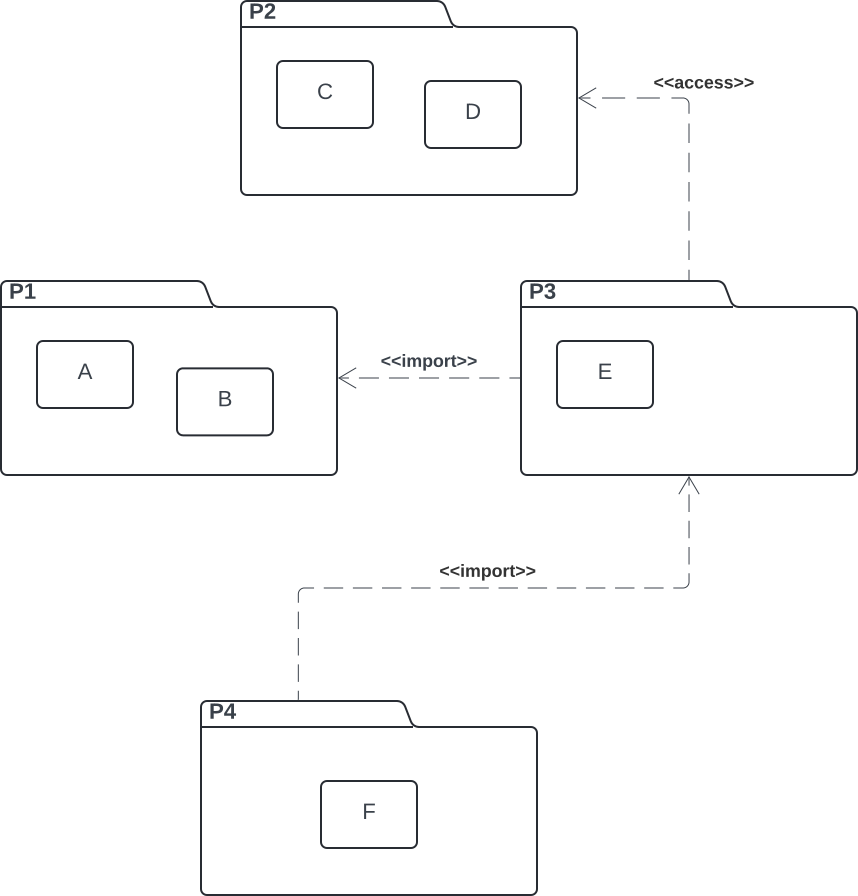
\includegraphics[scale=0.4]{part three/Klassendiagramme - Erweiterte Konzepte und Paketdiagramme/img/import-access}
    \caption{Verwendung von \guillemotleft import\guillemotright / \guillemotleft access\guillemotright in Paketdiagrammen. (Quelle: in Anlehnung an~\cite[308, Abb. 6.8-3]{Bal05})}
    \label{fig:import-access}
\end{figure}

\subsection{\guillemotleft merge\guillemotright}
Bei einem \textbf{merge} werden Elemente eines Zielpaketes in das Quellpaket kopiert und können dann verändert werden (vgl.~\cite[307]{Bal05}).\\
Durch einen Merge können Elemente gleichen Namens gemischt werden.
Abbildung~\ref{fig:import-merge} verdeutlicht dies: Das Zielpaket \code{Z} wird in Quellpaket \code{Q} \textit{gemergt}.
Unabhängig davon, ob \code{Q} bereits eine Klasse \code{A} oder \code{B} enthält, wird in \code{Q} jeweils eine Oberklasse \code{Z::A} bzw. \code{Z::B} eingefügt.
Existiert in \code{Q} keine Klasse \code{A} oder \code{B}, wird diese entsprechend eingefügt (vgl. \textit{einfacher Paket-Merge}, \cite[308]{Bal05}).


\begin{figure}
    \centering
    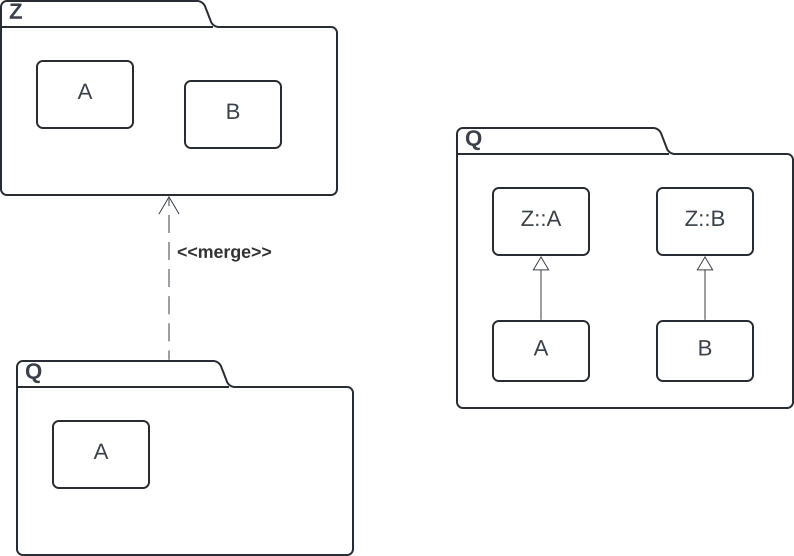
\includegraphics[scale=0.4]{part three/Klassendiagramme - Erweiterte Konzepte und Paketdiagramme/img/import-merge}
    \caption{Einfacher Paket-Merge. (Quelle: in Anlehnung an~\cite[308, Abb. 6.8-4]{Bal05})}
    \label{fig:import-merge}
\end{figure}